\section{Ergebnisse}
Die Zusammenfassung der Ergebnisse ist in \autoref{anh:ergebnisse} zu finden und umfasst vier Tabellen. Die Aufteilung in die vier Tabellen geschah entsprechend der Kompressionsverfahren, das bedeutet eine Tabelle enthält die Ergebnisse aller drei Kompressionsraten, aufgeteilt in die drei Datensätze und in die vier Analyseverfahren. Die ersten vier Werte entsprechen richtig positiv, richtig negativ, falsch positiv und falsch negativ, während die letzten beiden Werte für Sensitivität und Präzision stehen (siehe \autoref{sec:auswertung} für Bedeutungen und Abkürzungen). In dem folgenden Abschnitt sind diese Ergebnisse in vier Abbildungen mit jeweils drei Plots der F$_1$"=Maße aufgeteilt. Die Aufteilung geschah auch hier entsprechend der Kompressionsverfahren, das bedeutet in einer Abbildung findet sich ein Plot je Datensatz. Die x"=Achse eines Plots stellt die Kompressionsrate dar und die y"=Achse das F$_1$"=Maß. Die verschiedenfarbigen Linien zeigen die Entwicklung des F$_1$"=Maßes eines Analyseverfahrens, entlang sinkender Kompressionsrate. In zwei Plots sind nur drei Linien zu erkennen, was daran liegt, dass manche Verfahren identische Ergebnisse lieferten und somit sich überlagern. So in \autoref{subfig:f1linnvidia} die Verfahren knn und iForest und in \autoref{subfig:f1fouriernvidia} die Verfahren knn und Ähnlichkeitssuche.

In einem ersten Blick fällt auf, dass die Analyseverfahren zu einem großen Teil gut abschnitten. Dass bedeutet, dass in den meisten Fällen das F$_1$"=Maß über 0,7 lag und somit ein gutes Gleichgewicht zwischen Sensitivität und Präzision herrscht, egal welches Kompressionsverfahren und "=rate. Allerdings gibt es auch äußerst schlechte Ergebnisse, so zum Beispiel in \autoref{subfig:f1polecg}, wo nahezu alle Werte unter 0,5 liegen oder die Random Projection sogar dauerhaft F$_1$"=Maße von 0,0 oder leicht darüber besitzt. Generell fällt auch auf, dass die EKG"=Daten aus dem ECG5000 Datensatz am schlechtesten performen. So sind dort die meisten Werte unter 0,7 und schwanken auch um 0,7, was bedeutet, dass die Verfahren unterschiedlich gut beziehungsweise schlecht abschneiden. Bei den anderen beiden Datensätzen schwanken die Werte hingegen 

Schauen wir uns nun die Ergebnisse mit Fokus auf die Kompressionsverfahren an.


\begin{figure}[bth]
  \subfloat[Wetterdaten]{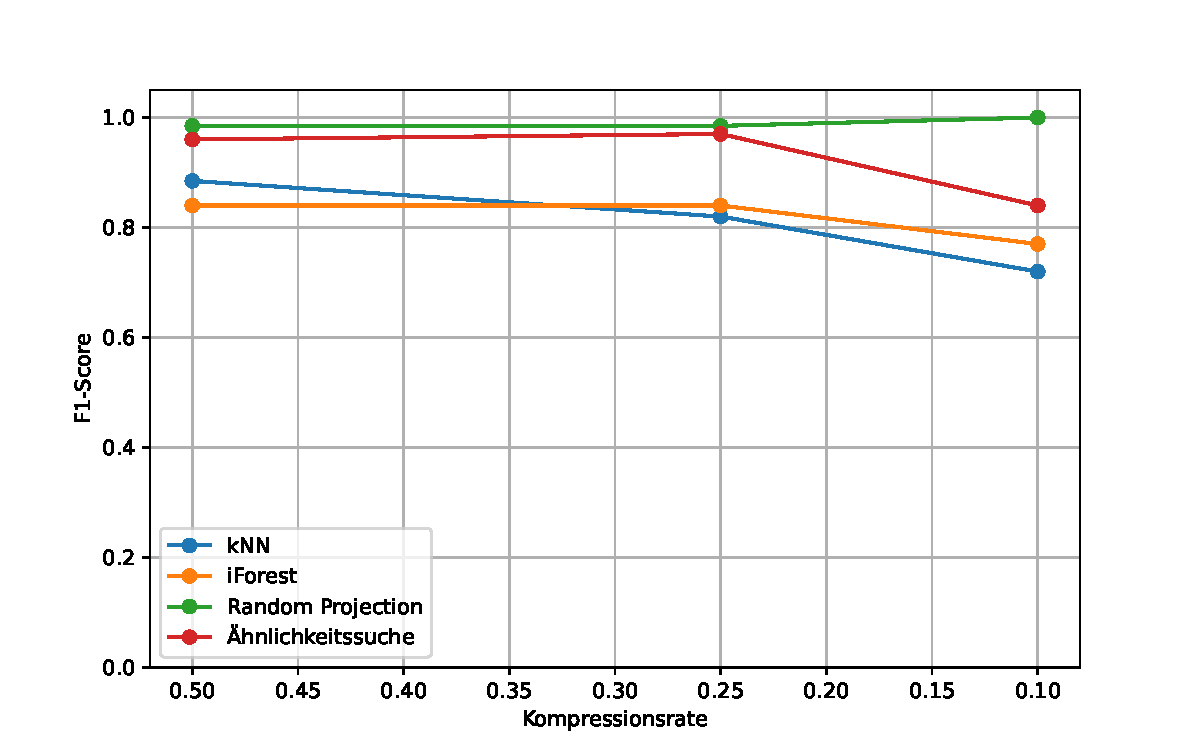
\includegraphics[width=0.49\textwidth]{Graphics/F1LinearWetter.pdf}\label{subfig:f1linwetter}}\hfill
  \subfloat[NVIDIA]{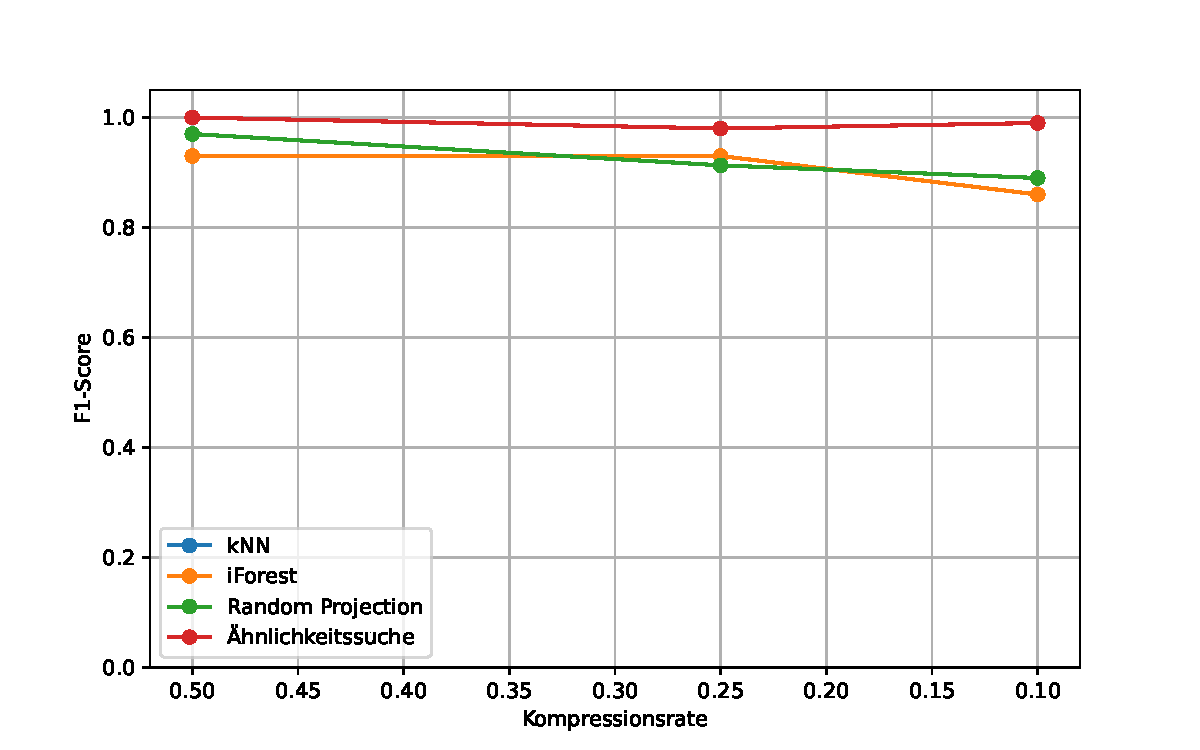
\includegraphics[width=0.49\textwidth]{Graphics/F1LinearNvidia.pdf}\label{subfig:f1linnvidia}}\hfill
  \centering\subfloat[ECG5000]{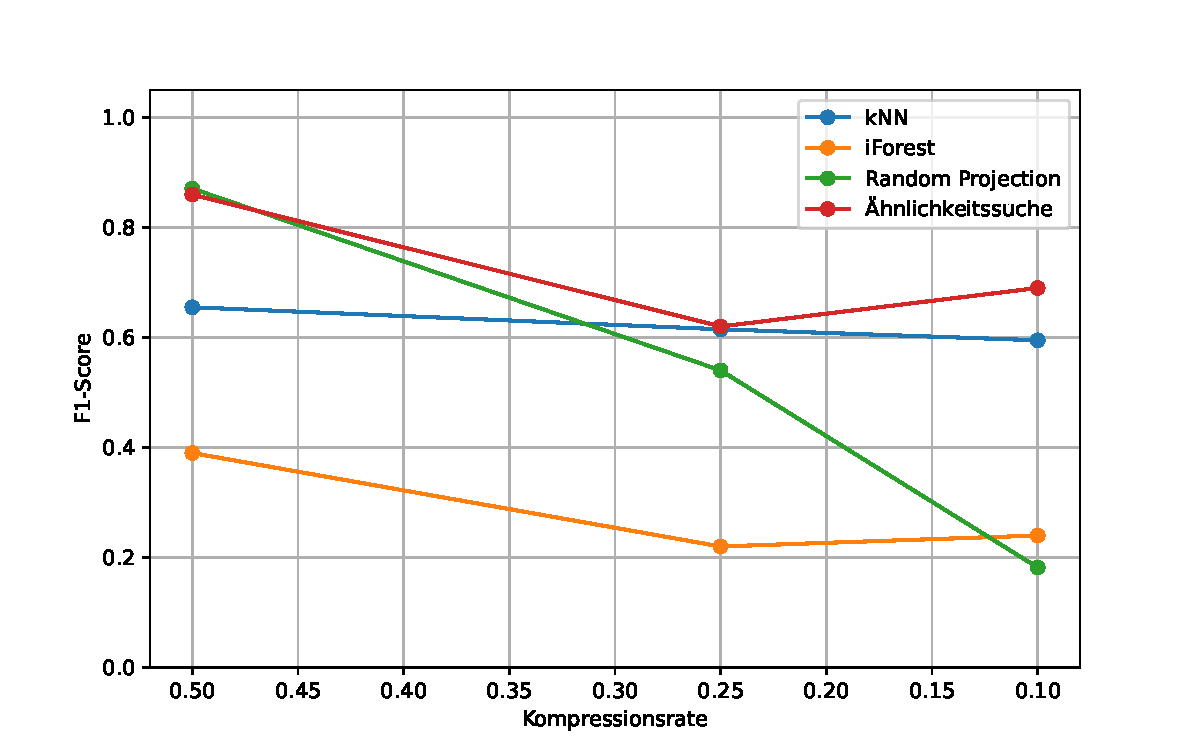
\includegraphics[width=0.49\textwidth]{Graphics/F1LinearECG.pdf}\label{subfig:f1linecg}}
  \caption{F1"=Maße der Analyseverfahren bei linearer Kompression}
  \label{fig:f1LinMaße}
\end{figure}

\begin{figure}[bth]
  \subfloat[Wetterdaten]{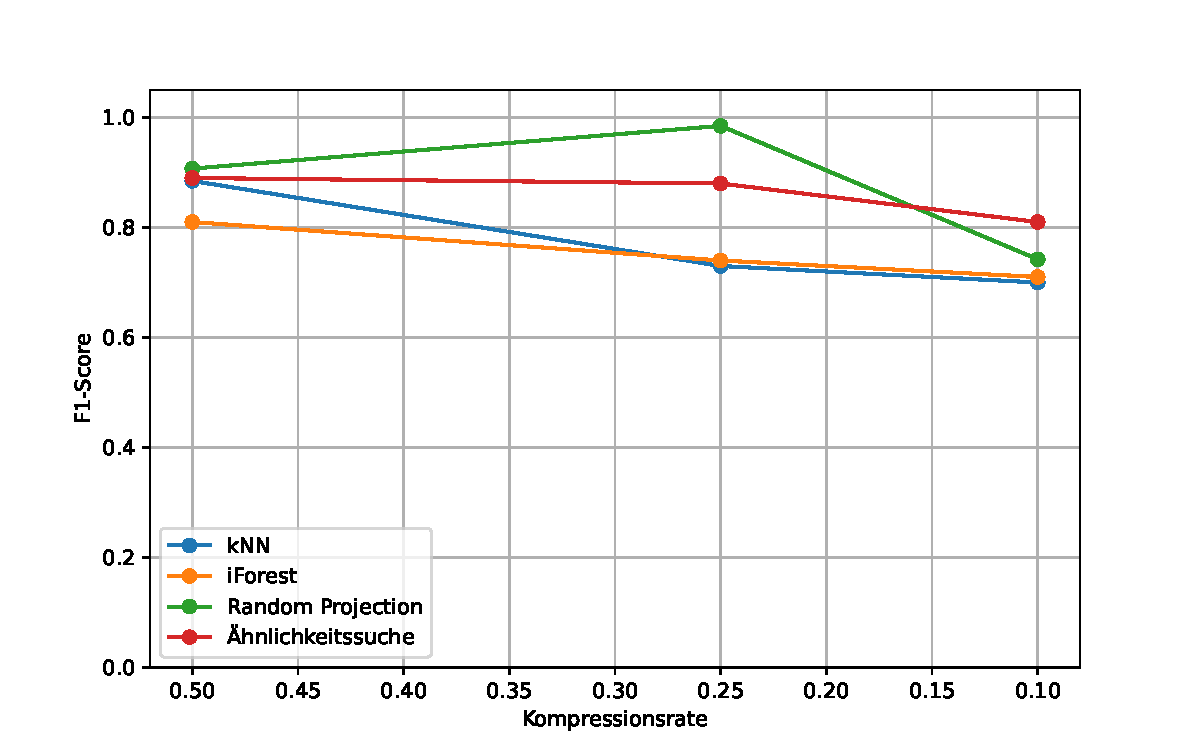
\includegraphics[width=0.49\textwidth]{Graphics/F1PolyWetter.pdf}\label{subfig:f1polwetter}}\hfill
  \subfloat[NVIDIA]{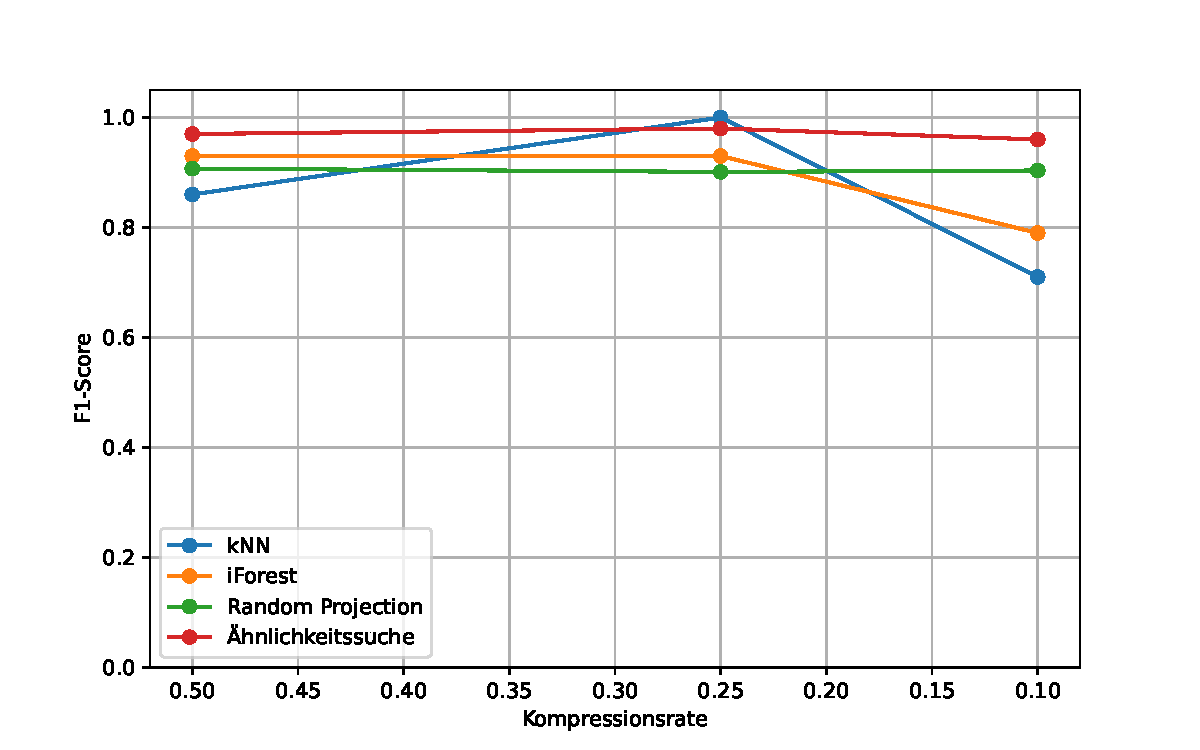
\includegraphics[width=0.49\textwidth]{Graphics/F1PolyNvidia.pdf}\label{subfig:f1polnvidia}}\hfill
  \centering\subfloat[ECG5000]{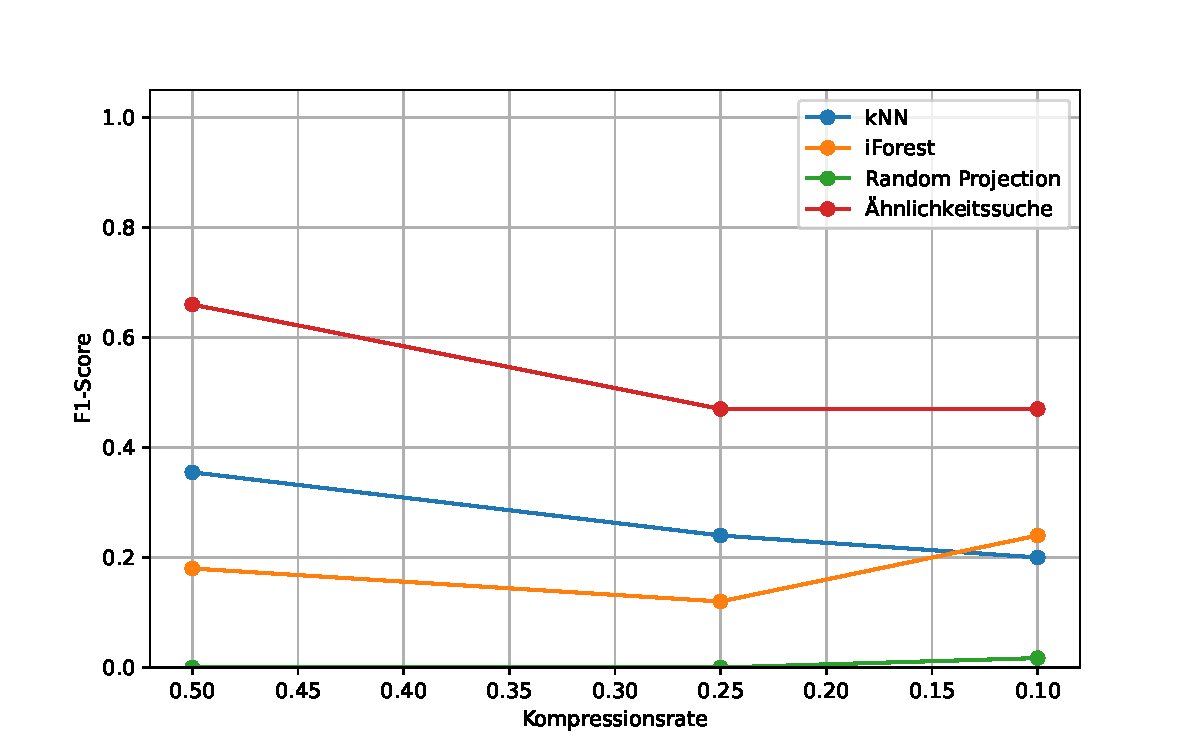
\includegraphics[width=0.49\textwidth]{Graphics/F1PolyECG.pdf}\label{subfig:f1polecg}}
  \caption{F1"=Maße der Analyseverfahren bei polynomieller Kompression}
  \label{fig:f1PolMaße}
\end{figure}

\begin{figure}[bth]
  \subfloat[Wetterdaten]{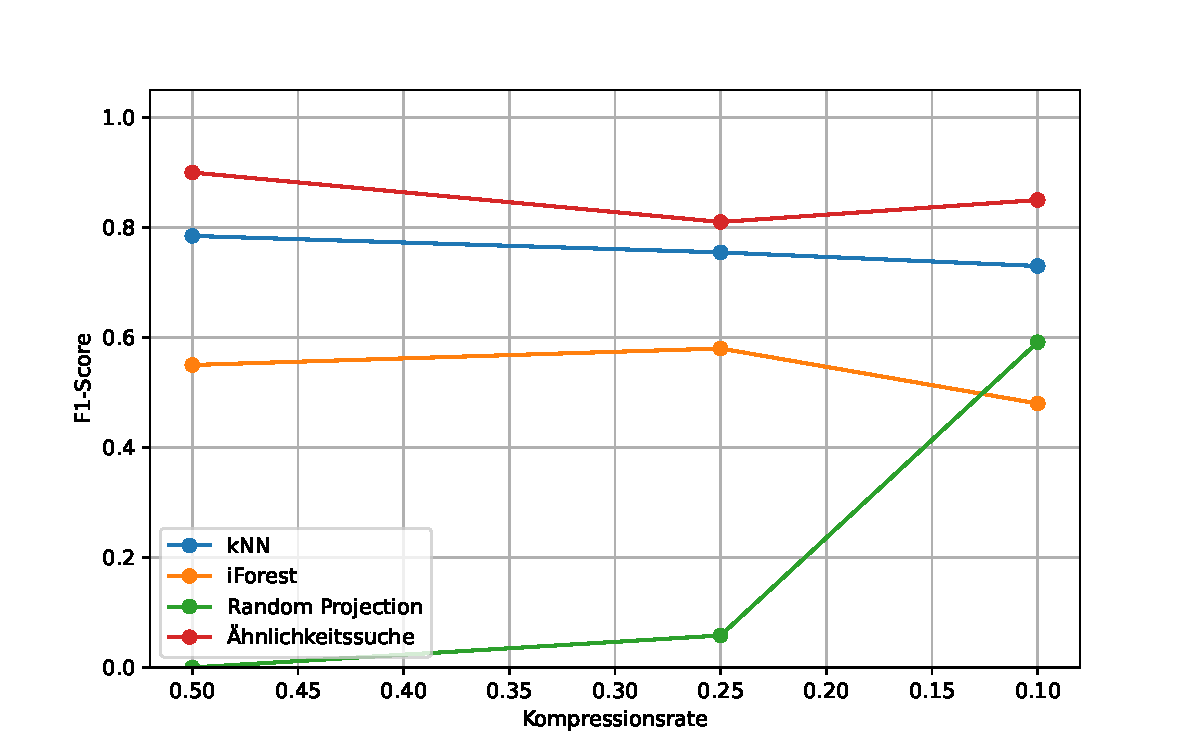
\includegraphics[width=0.49\textwidth]{Graphics/F1FourierWetter.pdf}\label{subfig:f1fourierwetter}}\hfill
  \subfloat[NVIDIA]{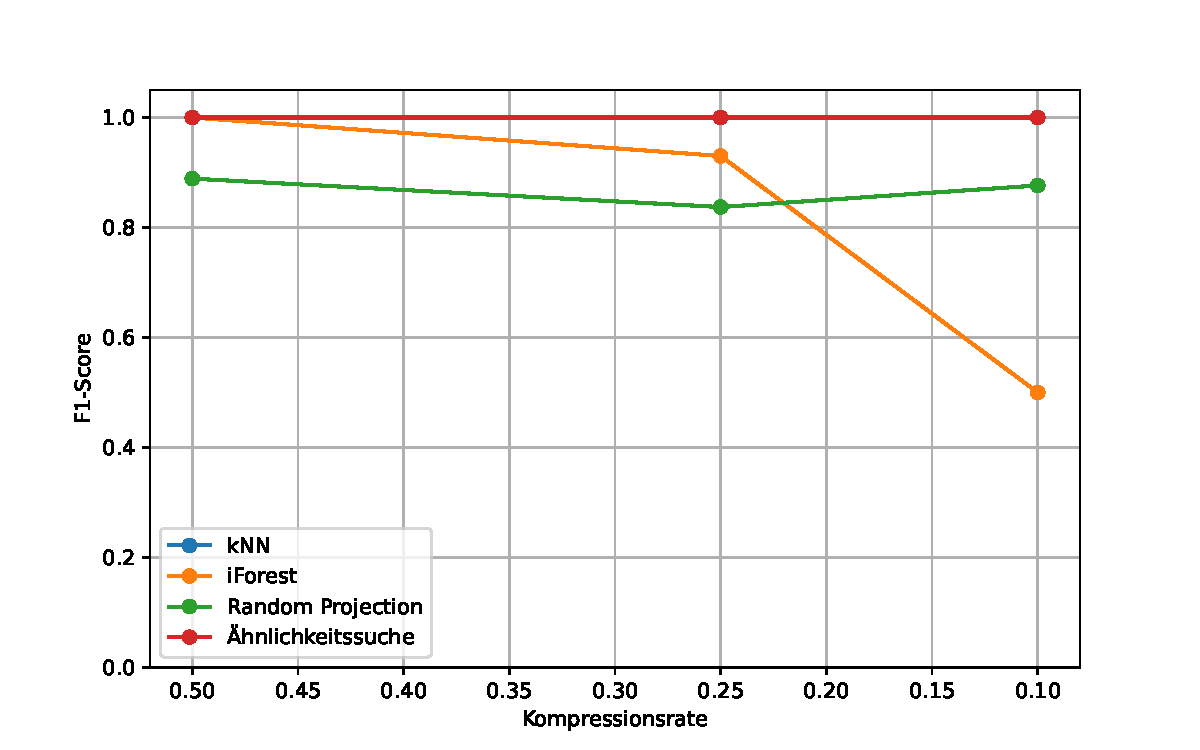
\includegraphics[width=0.49\textwidth]{Graphics/F1FourierNvidia.pdf}\label{subfig:f1fouriernvidia}}\hfill
  \centering\subfloat[ECG5000]{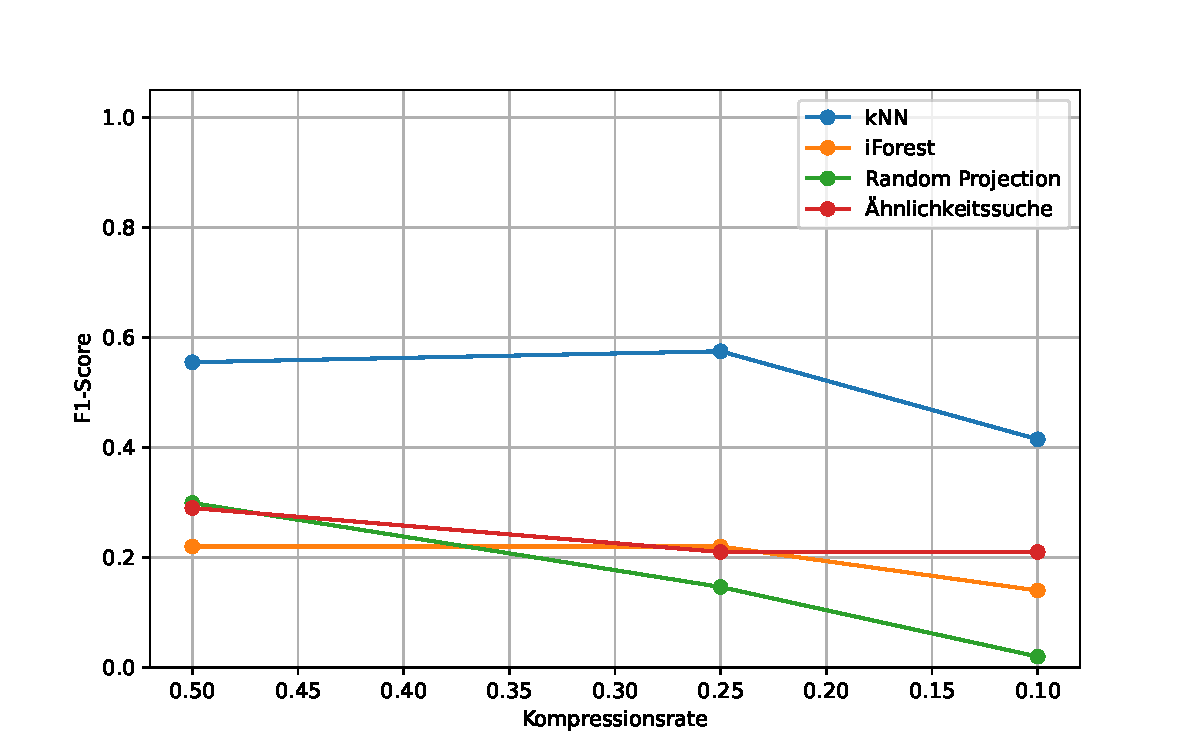
\includegraphics[width=0.49\textwidth]{Graphics/F1FourierECG.pdf}\label{subfig:f1fourierecg}}
  \caption{F1"=Maße der Analyseverfahren bei Fourier"=Kompression}
  \label{fig:f1FourMaße}
\end{figure}

\begin{figure}[bth]
  \subfloat[Wetterdaten]{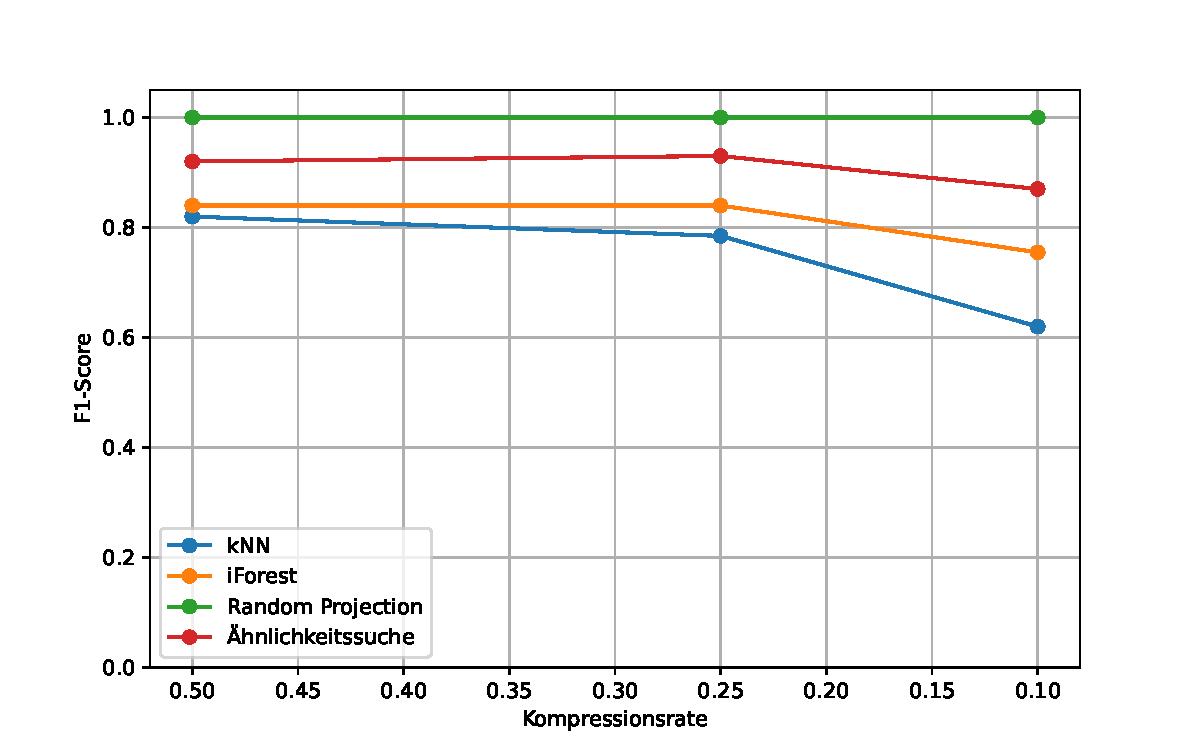
\includegraphics[width=0.49\textwidth]{Graphics/F1WaveletWetter.pdf}\label{subfig:f1waveletwetter}}\hfill
  \subfloat[NVIDIA]{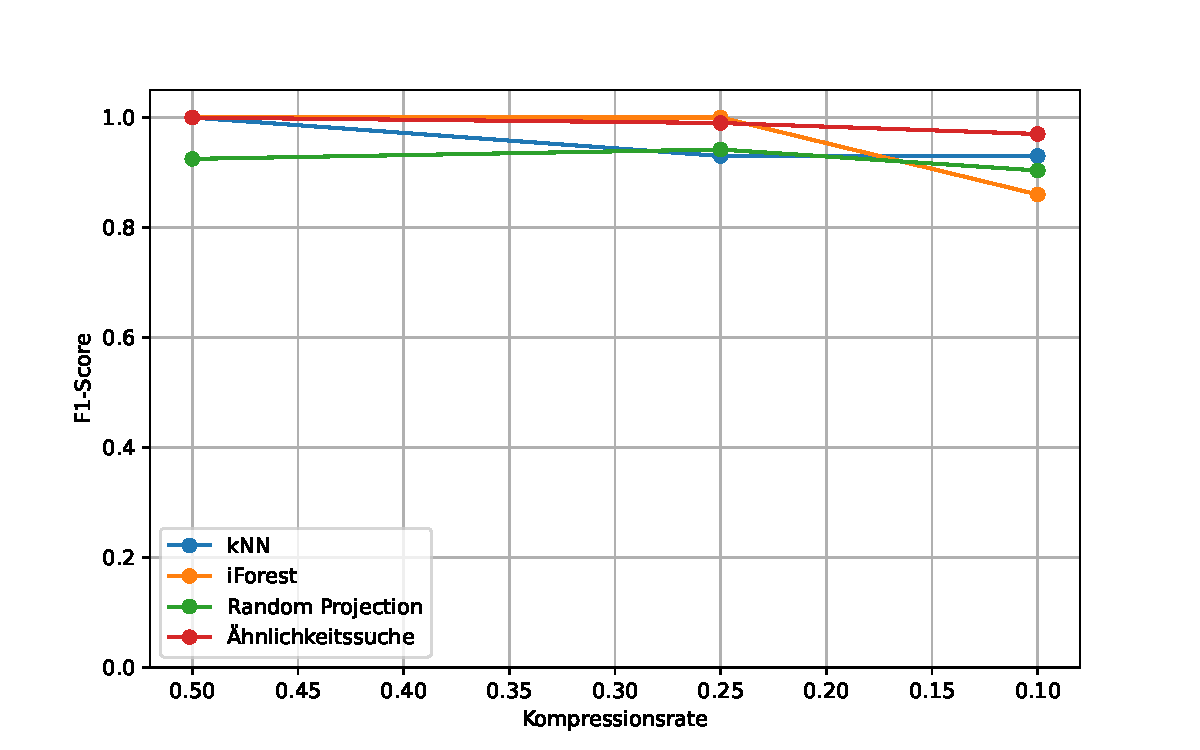
\includegraphics[width=0.49\textwidth]{Graphics/F1WaveletNvidia.pdf}\label{subfig:f1waveletnvidia}}\hfill
  \centering\subfloat[ECG5000]{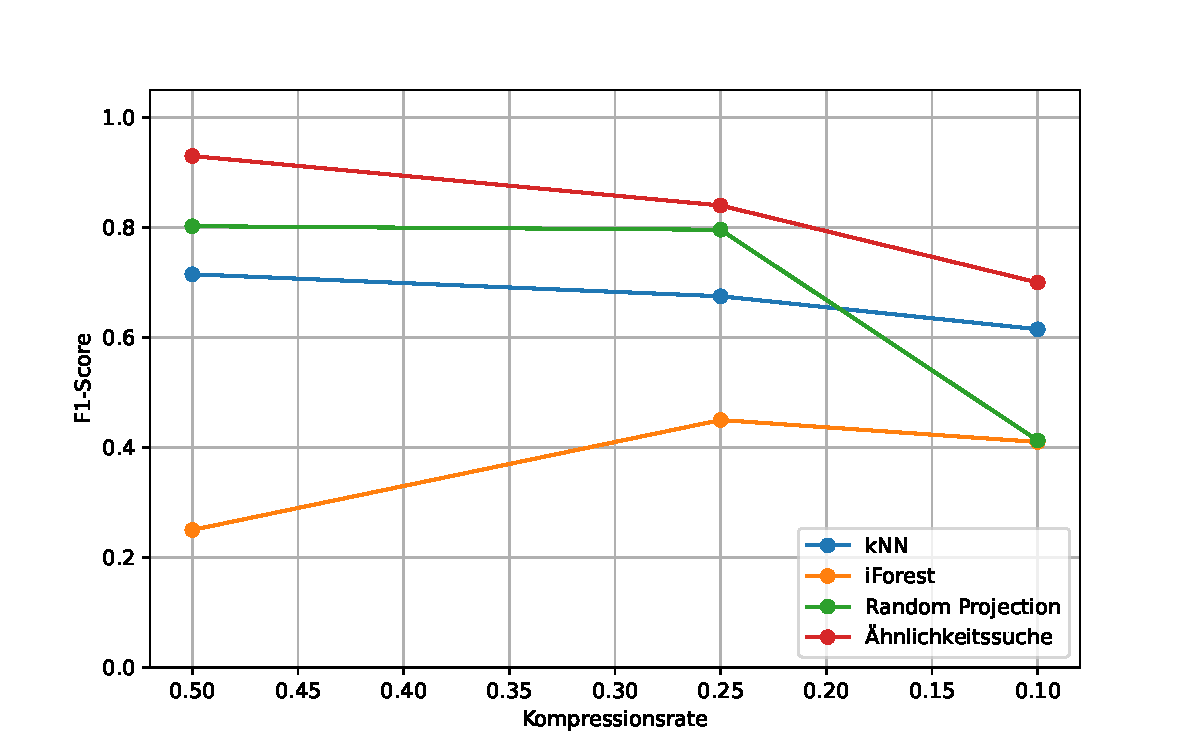
\includegraphics[width=0.49\textwidth]{Graphics/F1WaveletECG.pdf}\label{subfig:f1waveletecg}}
  \caption{F1"=Maße der Analyseverfahren bei Wavelet"=Kompression}
  \label{fig:f1WaveletMaße}
\end{figure}

% Linear Laufzeit
\begin{table}[t]
 \centering
 \begin{tabular}{lc|cccc}
  \toprule
  \multicolumn{1}{c}{\bfseries Daten} & \boldmath $\rho$ & \bfseries knn & \bfseries iForest & \bfseries Random P. & \bfseries Ähnlichkeitss. \\ 
  \midrule
   \multirow{3}{*}{Wetterdaten} & 0,50 & \tabledata{12,35}{1,69}{5,94}{6,59}
   & 0,25 & \tabledata{15,45}{1,84}{10,68}{12,98}
   & 0,10 & \tabledata{15,09}{1,91}{16,56}{27,03}
   \midrule
   \multirow{3}{*}{NVIDIA-Aktie} & 0,50 & \tabledata{13,57}{1,03}{1,41}{2,05}
   & 0,25 & \tabledata{17,50}{1,56}{1,59}{2,84}
   & 0,10 & \tabledata{34,77}{1,56}{1,84}{4,23}
   \midrule
   \multirow{3}{*}{ECG5000} & 0,50 & \tabledata{7,26}{1,18}{2,40}{2,84}
   & 0,25 & \tabledata{9,31}{1,24}{3,40}{4,99}
   & 0,10 & \tabledata{8,53}{1,73}{4,28}{8,80}
  \bottomrule
 \end{tabular}
 \caption{Prozentuale Steigerung der Laufzeit bei Linearer Kompression}
\end{table}

% Poly Laufzeit
\begin{table}[t]
 \centering
 \begin{tabular}{lc|cccc}
  \toprule
  \multicolumn{1}{c}{\bfseries Daten} & \boldmath $\rho$ & \bfseries knn & \bfseries iForest & \bfseries Random P. & \bfseries Ähnlichkeitss. \\ 
  \midrule
   \multirow{3}{*}{Wetterdaten} & 0,50 & \tabledata{13,73}{1,70}{6,20}{6,89}
   & 0,25 & \tabledata{17,17}{1,85}{10,97}{13,57}
   & 0,10 & \tabledata{17,93}{1,92}{17,23}{30,45}
   \midrule
   \multirow{3}{*}{NVIDIA-Aktie} & 0,50 & \tabledata{14,24}{1,03}{1,34}{1,95}
   & 0,25 & \tabledata{19,56}{1,56}{1,56}{2,85}
   & 0,10 & \tabledata{40,12}{1,57}{1,84}{4,41}
   \midrule
   \multirow{3}{*}{ECG5000} & 0,50 & \tabledata{7,26}{1,19}{2,39}{2,84}
   & 0,25 & \tabledata{14,84}{1,24}{3,40}{4,96}
   & 0,10 & \tabledata{12,77}{1,73}{4,31}{9,00}
  \bottomrule
 \end{tabular}
 \caption{Prozentuale Steigerung der Laufzeit bei polynomieller Kompression}
\end{table}

% Fourier Laufzeit
\begin{table}[t]
 \centering
 \begin{tabular}{lc|cccc}
  \toprule
  \multicolumn{1}{c}{\bfseries Daten} & \boldmath $\rho$ & \bfseries knn & \bfseries iForest & \bfseries Random P. & \bfseries Ähnlichkeitss. \\ 
  \midrule
   \multirow{3}{*}{Wetterdaten} & 0,50 & \tabledata{7,68}{1,47}{2,95}{3,12}
   & 0,25 & \tabledata{12,53}{1,70}{5,67}{6,35}
   & 0,10 & \tabledata{11,32}{1,80}{7,90}{9,11}
   \midrule
   \multirow{3}{*}{NVIDIA-Aktie} & 0,50 & \tabledata{14,88}{1,02}{1,32}{1,78}
   & 0,25 & \tabledata{12,11}{1,03}{1,31}{1,83}
   & 0,10 & \tabledata{18,72}{1,03}{1,32}{1,95}
   \midrule
   \multirow{3}{*}{ECG5000} & 0,50 & \tabledata{5,46}{1,11}{1,69}{1,85}
   & 0,25 & \tabledata{10,24}{1,17}{2,01}{2,24}
   & 0,10 & \tabledata{5,38}{1,20}{3,47}{5,53}
  \bottomrule
 \end{tabular}
 \caption{Prozentuale Steigerung der Laufzeit bei Fourier"=Kompression}
\end{table}

% Wavelet Laufzeit
\begin{table}[t]
 \centering
 \begin{tabular}{lc|cccc}
  \toprule
  \multicolumn{1}{c}{\bfseries Daten} & \boldmath $\rho$ & \bfseries knn & \bfseries iForest & \bfseries Random P. & \bfseries Ähnlichkeitss. \\ 
  \midrule
   \multirow{3}{*}{Wetterdaten} & 0,50 & \tabledata{14,33}{1,71}{6,32}{7,04}
   & 0,25 & \tabledata{19,49}{1,83}{10,19}{12,24}
   & 0,10 & \tabledata{19,54}{1,92}{18,48}{35,26}
   \midrule
   \multirow{3}{*}{NVIDIA-Aktie} & 0,50 & \tabledata{14,27}{1,03}{1,32}{1,93}
   & 0,25 & \tabledata{18,02}{1,57}{1,56}{2,72}
   & 0,10 & \tabledata{38,52}{1,57}{1,84}{4,39}
   \midrule
   \multirow{3}{*}{ECG5000} & 0,50 & \tabledata{7,52}{1,18}{2,56}{3,12}
   & 0,25 & \tabledata{16,67}{1,24}{3,53}{5,42}
   & 0,10 & \tabledata{7,92}{1,73}{4,20}{8,49}
  \bottomrule
 \end{tabular}
 \caption{Prozentuale Steigerung der Laufzeit bei Wavelet"=Kompression}
\end{table}